\section{Введение}
\subsection{Актуальность работы}
Кровь -- это соединительная ткань внутри организма, она состоит из форменных элементов (эритроцитов, лейкоцитов, тромбоцитов), 
а так же водного раствора белков и свёртывающих веществ -- плазмы. Объёмная доля форменных элементов в общем объеме называется 
гематокритом и составляет примерно 45\%.
Функций у крови несколько: она является транспортным средством, поддерживает постоянство <<внутренней среды>> организма (гомеостаз), 
играет главную роль в защите от чужеродных веществ.

\begin{figure}[h]
\centering
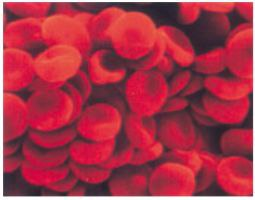
\includegraphics[width=0.3\linewidth]{erotr.jpg}
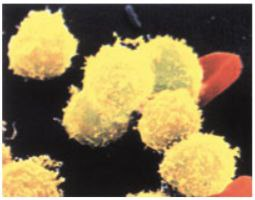
\includegraphics[width=0.3\linewidth]{leiko.jpg}
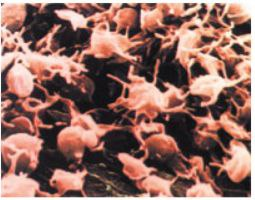
\includegraphics[width=0.3\linewidth]{trombo.jpg}
\caption{ Электронные фотографии элементов крови: 1 -- эритроциты, 2 -- лейкоциты, 3 -- тромбоциты~\cite{rls:2003}}.
\label{fig:mpr}
\end{figure}
С развитием медицины и науки в целом, появилась необходимость в изучении течения крови. Зная как движется кровь в организме, 
мы получаем более масштабную картину того, как работает наш организм, можем помочь поставить диагноз, спрогнозировать развитие 
заболеваний, подобрать оптимально лечение.

В изучении течения крови не малую роль играет вычислительная гидродинамика. Её главное достоинство -- возможность проводить практически 
неограниченное количество численных экспериментов без опасности для жизни и здоровья испытуемого. Так же вычислительная гидродинамика 
позволяет моделировать сложные процессы, недоступные аналитическим методам гидродинамики и получать такие параметры течений, которые 
сложно или невозможно получить в реальном эксперименте.

\subsection{Общее описание течения крови в организме}
Кровь движется по замкнутой системе сосудов, циркулируя от сердца и обратно. Кровеносная система человека -- сложная, разветвленная сеть,
состоящая из вен, артерий и капилляров.
Диаметры сосудов варьируются от \texttilde$15.3\cdot 10^{-3}$~м (для самого крупного артериального сосуда -- аорты)
до \texttilde$8\cdot 10^{-6}$~м (для мелких капилляров).

Кровь движется по сосудам под воздействием периодических сокращений сердечной мышцы, описываемых сердечным циклом. 
Под сердечным циклом понимают период, охватывающий одно сокращение и одно расслабление предсердий и желудочков. 
Общая длительность сердечного цикла при частоте сердечных сокращений 75~уд/мин равна 0.8~с. Систола (0.33~с) -- фаза сердечного цикла, 
включающая сокращение миокарда и изгнание крови из сердца в сосудистую систему. Диастола (0.47~c) -- фаза сердечного цикла, 
включающая расслабление миокарда и наполнение полостей сердца кровью.

\begin{figure}[h!]
    \centering
    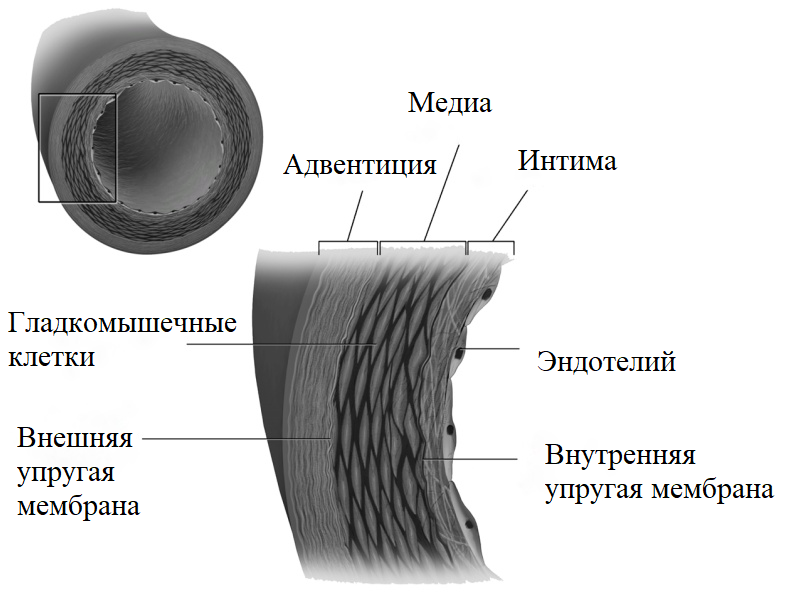
\includegraphics[width=0.4\linewidth]{stenki2.png}
    \caption{Типовое строение стенки кровеносного сосуда ~\cite{blausen:2014}}
    \label{tip}
    \end{figure}

Стенку кровеносного сосуда (за исключением капилляров) условно можно разделить на три слоя: интима -- внутренний слой, 
медиа -- средний слой, адвентиция -- внешний слой (Рис.~\ref{tip}).
В зависимости от состава сосудистой стенки, артерии условно делят на эластичный или мышечный типы. 
Артерии эластичного типа -- сосуды относительно большого диаметра, расположенные ближе к сердцу (например аорта), 
медиа которых содержит большое количество упругих мембран. Число упругих мембран убывает при уменьшении размера сосуда. 
Они практически отсутствуют в артериях мышечного типа. Артерии мышечного типа находятся на периферии (например, бедренная артерия). 
В среднем слое артерий мышечного типа доминируют гладкомышечные клетки. Вены, в отличие от артерий, делятся по размеру внутреннего 
диаметра. У вен толщина стенок и толщина среднего слоя намного меньше, чем у артерий. При этом у вен толще внешний слой ~\cite{Rhodin:1980}. 

Кровообращение состоит из двух кругов. Течение крови по малому кругу начинается в правом желудочке, при сокращении которого венозная кровь попадает в легочный ствол и, 
протекая через легкие, отдает диоксид углерода и насыщается кислородом. Обогащенная кислородом кровь из легких по легочным венам 
поступает в левое предсердие, где заканчивается малый круг. Большой круг начинается в левом желудочке, при сокращении которого кровь, 
обогащенная кислородом, нагнетается в аорту, артерии, артериолы и капилляры всех органов и тканей, а оттуда по венулам и венам 
притекает в правое предсердие, где и заканчивается большой круг.

\begin{figure}[h!]
    \centering
    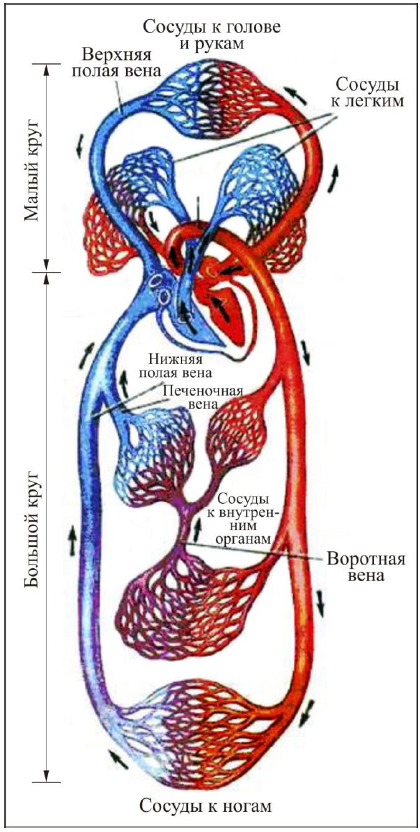
\includegraphics[width=0.3\linewidth]{screenshot_2.png}
    \caption{Общая схема кровообращения человека.}
    \label{tip}
    \end{figure}

Кровь, двигаясь по сосудам, испытывает сопротивление движению из-за своей вязкости и со стороны сосудов. 
Величина сопротивления зависит от диаметра сосуда, его длины, скорости кровотока. Поэтому сердце выбрасывает кровь 
в сосудистую систему под большим давлением. В разных отделах сосудистой системы давление крови будет разным. 
В аорте среднее давление в 100~мм рт.ст. колеблется в диапазоне от 120~мм рт.ст. при систоле до 80~мм рт.ст. при диастоле. 
Разница между ними -- пульсовое давление. По мере движения крови давление в сосудистом русле падает. Таким образом, непрерывные, 
ритмические сокращения сердца, преодолевая сопротивление, создают и поддерживают разность кровяного давления между артериальным и 
венозным участком сосудистой системы, тем самым приводя кровь в движение.


\begin{figure}[h!]
    \centering
    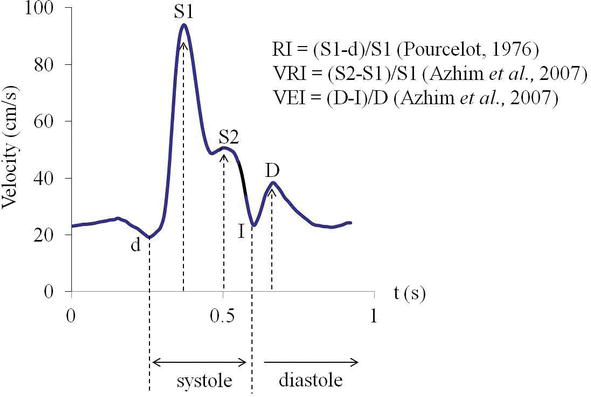
\includegraphics[width=0.7\linewidth]{doppler.png}
    \caption{Значение скорости кровотока в аорте на различных фазах сердечного ритма~\cite{Azhim18}.}
    \label{velosit}
    \end{figure}
Скорость течения крови существенно отличается для разных типов сосудов. Она зависит от диаметра сосуда, удалённости сосуда от сердца,
а также фазы сердечного цикла (Рис.~\ref{velosit}). Максимальных значений скорость достигает в аорте (до \texttilde$1$~м/с), а минимальных --
в капиллярах (около нуля).
Линейная скорость в полых венах в два раза меньше, 
чем в аорте и равна примерно $2.5\cdot10^{-1}$~м/с, поскольку в организме на одну артерию приходится две вены. 

Вязкость крови обычно оценивают в 4.3 -- 4.9~мПа$\cdot$с, а её плотность -- в 1052 -- 1060~кг/м\textsuperscript{3}. 
В зависимости от наличия заболеваний, определенного образа жизни и питания эти показатели могут отходить от нормы. 

Гидродинамические характеристики зависят от режима течения, который определяется числом Рейнольдса
$$\Ren=\frac{v\cdot D\cdot \rho}{\mu}$$,
где $v$ -- скорость течения жидкости, $D$ -- радиус трубы, $\rho$ -- плотность жидкости, $\mu$ -- вязкость жидкости.
Исходя из определённых параметров течения можно оценить максимальное характерное число Рейнольдса для течений в аорте, как
$\Ren\approx 1000 $. Число Рейнольдса, при котором начинается процесс ламинарно-турбулентного перехода, называется критическим.  
Для гладких труб критическое число Рейнольдса известно из многочисленных экспериментов и численных исследований. В среднем оно равно $\Ren^*=2300$.
Таким образом, можно сделать вывод, что движение крови в организме в основном ламинарное. 
Однако, при определенных условиях, кровоток может приобретать и турбулентный характер.
Турбулентность проявляется в полостях сердца (велико значение $A$), вблизи клапанов сердца (высокая скорость движения крови). 
При интенсивной физической нагрузке скорость движения крови увеличивается, и это может вызвать турбулентность в кровотоке. 
При некоторых патологических процессах, приводящих к аномальному снижению вязкости крови, кровоток в крупных кровеносных сосудах может 
стать турбулентным.  При наличии атеросклеротических бляшек в просвете сосудов имеются локальные сужения, приводящие к возникновению 
турбулентности в течении крови. 


Состоит кровь, как уже было сказано ранее, из форменных клеток и плазмы. Значение гематокрита варьируется в зависимости от пола,
возраста в границах 0.37 -- 0.54. 99 \% гематокрита 
приходится на эритроциты. Эритроциты -- двояковогнутые диски, размерами 7 -- 8~мкм, их количество так же зависит
от параметров организма 
и варьируется от 3.8 до 5.6 миллиардов клеток на 1~см$^3$. 
Лейкоциты -- ядерные клетки округлой формы, их количество на 1~см$^3$ составляет 4.5 -- 11 миллионов, а размеры 4 -- 20~мкм, 
количество тромбоцитов 150 -- 400 миллионов на 1~см$^3$ и размеры 2 -- 4~мкм. 60 \% от объёма крови приходится на плазму -- жидкое межклеточное 
вещество, содержащее 90 -- 93 \% воды и 7 -- 10 \% сухого вещества (белки, углеводы, соли).

\subsection{Вывод}
 С точки зрения гидродинамики кровоток представляет из себя пульсирующее с низкой частотой течение мелкодисперсной суспензии в 
 замкнутой системе каналов кругового сечения с эластичными стенками, осложнённое локальными эффектами ламинарно-турбулентного перехода.
